% Do not remove the next line
% Synchronized to r34917

\marklabel{chap:bootmedien}{
  \chapter{Création une archive fli4l/Média de Boot}
  }

  Lorsque tous les fichiers de configuration seront paramétrés,
  l'archive fli4l/Média de Boot peut être construite, on peut
  soit utiliser une carte Compact Flash pour booter ou créer une image ISO,
  soit uniquement faire une mise à jour des fichiers.


\marklabel{sec:bootmedien_linux}{
  \section{Création de l'archive fli4l/Média de Boot sous Linux, dérivé Unix
  et Mac OS X}
  }

  La construction se fait à l'aide du Scripts (\texttt{.sh}) qui se trouve
  dans la racine du répertoire de fli4l.

  \begin{description}
    \item \texttt{mkfli4l.sh}
  \end{description}

  Build-Script (ou script de construction) reconnaît indépendamment
  les différentes \jump{BOOTTYPE}{variantes de Boot}.

  La simple commande sous Linux est~:
  \begin{verbatim}
    sh mkfli4l.sh
  \end{verbatim}

  Les trois mécanismes suivant gèrent le démarrage de Build-Scripts~:
  \begin{itemize}
    \item La configuration de la variable \var{BOOT\_TYPE} dans le
          fichier \texttt{$<$config$>$/base.txt}
    \item La configuration du fichier \texttt{$<$config$>$/mkfli4l.txt}
    \item Les paramètres du Build-Scripts
  \end{itemize}

  On décide au moyen de la variable \jump{BOOTTYPE}{\var{BOOT\_TYPE}},
  le type de support de construction (Build-Scripts) pour fli4l~:
  \begin{itemize}
    \item Démarrer fli4l avec un CD-ROM par une image ISO
    \item Faire une mise à jour des fichiers, pour une nouvelle
      version fli4l
    \item Créer les fichiers fli4l et faire une mise à jour à distance via SCP
    \item etc.
  \end{itemize}

  Vous trouverez la description des variables dans le fichier de
  configuration \texttt{$<$config$>$/mkfli4l.txt} et dans le chapitre
  \jump{sec:mkfli4lconf}{Paramètres mkfli4l.txt}.


  \subsection{Lignes de commandes optionnelle}

  Les mécanismes de contrôle sont à ajouter aux paramètres d'option
  lorsque vous appelez le script de compilation par ligne de commande.
  Les options de contrôle sont semblables à ceux du fichier de commande \texttt{mkfli4l.txt}.
  Les spécifications des paramètres d'options remplacent les valeurs du fichier
  de contrôle. Pour des raisons de confort on a différencié, les paramètres
  optionnels et les variables du fichier de construction. les paramètre existe
  sous une forme courte et longue~:

  \begin{verbatim}
Utiliser : mkfli4l.sh [options] [config-dir]

-c, --clean             cleanup the build-directory
-b, --build <dir>       sets build-directory to <dir> for the fli4l-files
-v, --verbose           verbose - some debug-output
    --filesonly         creates only fli4l-files - does not create a boot-media
    --no-squeeze        don't compress shell scripts
-h, --help              display this usage

config-dir              sets other config-directory - default is "config"

--hdinstallpath <dir>   install a pre-install environment directly to
                    usb/compact flash device mounted or mountable to
                    directory <dir> in order to start the real installation
                    process directly from that device
                    device either has to be mounted and to be writable
                    for the user or it has to be mountable by the user
                    Do not use this for regular updates!

*** Remote-Update options
--remoteupdate          remote-update via scp, implies "--filesonly"
--remoteremount         make /boot writable before copying files and
                        read only afterwards
--remoteuser <name>     user name for remote-update - default is "fli4l"
--remotehost <host>     hostname or IP of remote machine - default
                        is HOSTNAME set in [config-dir]/base.txt
--remotepath <path>     pathname on remote maschine - default is "/boot"
--remoteport <portnr>   portnumber of the sshd on remote maschine

*** Netboot options
--tftpbootpath <path>   pathname to tftpboot directory
--tftpbootimage <name>  name of the generated bootimage file
--pxesubdir <path>      subdirectory for pxe files relative to tftpbootpath

*** Developer options
-u, --update-ver    set version to <fli4l_version>-rev<svn revision>
-v, --verbose       verbose - some debug-output
-k, --kernel-pkg    create a package containing all available kernel
                    modules and terminate afterwards.
                    set COMPLETE_KERNEL='yes' in config-directory/_kernel.txt
                    and run mkfli4l.sh again without -k to finish
    --filesonly     create only fli4l-files - do not create a boot-media
    --no-squeeze    don't compress shell scripts
    --rebuild       rebuild mkfli4l and related tools; needs make, gcc
  \end{verbatim}

  Avec l'option \verb+--hdinstallpath <dir>+ il est possible de faire une
  pré-installation sur une carte compact-flash en utilisant un lecteur de carte
  USB ou sur une clé USB, les supports doivent être formater en (FAT16/FAT32).
  Cette fonction est surtout utilisée \emph{à vos propres risques} pour la
  création de carte compact-flash ou de clé USB. Les fichiers nécessaires pour
  fli4l seront copiés sur la partition spécifiée. Le script ci-dessous appelle
  le répertoire fli4l.

  \begin{verbatim}
     sh mkfli4l.sh --hdinstallpath <dir>
  \end{verbatim}
  \vspace{-2ex}

  Les fichiers fli4l seront copiés sur la carte CF ou sur la clé USB.

  Pour effectuer les prochaines étapes, les conditions suivantes doivent être remplies~:

   \begin{itemize}
        \item \verb+chmod 777 /dev/brain+
        \item Droits-super-utilisateur
        \item Installer \verb+syslinux+
        \item Installer \verb+fdisk+
   \end{itemize}

  Ensuite le script contrôle, si le support de données est un lecteur USB et si
  la première partition est une partition FAT. Puis le Bootloader et les fichiers
  nécessaires sont copiés sur le volume spécifié. A la fin du script, vous
  recevrez un message indiquant le succès ou l'échec de l'installation.

  Après la construction, vous devez exécuter.

 \begin{verbatim}
 syslinux --mbr /dev/brain

    # make partition bootable using fdisk
    #     p - print partitions
    #     a - toggle bootable flag, specify number of fli4l partition
    #         usually '1'
    #     w - write changes and quit
    fdisk /dev/brain

    # install boot loader
    syslinux -i /dev/brain
 \end{verbatim}
 \vspace{-2ex}

  Pour finir, la carte CF ou la clé USB sera amorçable. Ne pas oublier de
  démonter le périphérique (avec \texttt{umount}).

  \bigskip

  Avec les derniers paramètres d'optionnel, On peut créer un répertoire
  de configuration alternatif. Le répertoire de configuration normal s'appelle
  \texttt{config} et se trouve directement à la racine du répertoire de fli4l.
  Dans ce répertoire, sont enregistrés tous les fichiers de configuration des
  paquetages fli4l. Si on veut gérer plus d'une configuration, on peut créer un
  répertoire supplémentaire, par exemple \texttt{hd.conf}, ici une copie des
  fichiers de configuration est faite et si vous voulez vous pouvez modifies
  ces fichiers selon vos besoins. Quelque exemples~:
  \begin{verbatim}
     sh mkfli4l.sh --filesonly hd.conf
     sh mkfli4l.sh --no-squeeze config.test
  \end{verbatim}


\marklabel{sec:bootmedien_windows}{
  \section{Création d'une archive fli4l/Média de Boot sous Windows}
  }

  Le programme utilisé est 'AutoIt3' voir le site
  (\altlink{http://www.autoitscript.com/site/autoit/}). il permet une construction
  'graphique' de fli4l et aussi des dialogues dans lesquels les variables
  sont décrites dans ce paragraphe, voici la commande.

  \begin{description}
    \item \texttt{mkfli4l.bat}
  \end{description}

  Build-Script reconnaît indépendamment les différentes \jump{BOOTTYPE}{variantes de Boot}.

  Le démarrage de 'mkfli4l.bat' peut s'opérer directement dans
  l'Explorer de Windows, sans utiliser aucun paramètre optionnel.

  Les différents mécanismes gérent la construction du programme Build~:
  \begin{itemize}
    \item Configuration de la variable \var{BOOT\_TYPE} dans
      le fichier \texttt{$<$config$>$/base.txt}
    \item Configuration du fichier \texttt{$<$config$>$/mkfli4l.txt}
    \item Les Paramètres du Programme Build
    \item Le Réglage interactif avec le GUI
  \end{itemize}

  On décide au moyen de la variable \jump{BOOTTYPE}{\var{BOOT\_TYPE}},
  le type de média de construction (Build-Scripts) pour fli4l~:
  \begin{itemize}
    \item Démarrer fli4l avec un CD-ROM par une image ISO
    \item Faire une mise à jour des fichiers, les copier sur le média
    \item Faire une mise à jour des fichiers, les envoyer sur le routeur via SCP
    \item Pré-installer un Disque Dur ou un CF (Compact Flash) en
      utilisent un lecteur de carte
    \item etc.
  \end{itemize}

  Vous trouverez la description des variables dans le fichier de
  configuration \texttt{$<$config$>$/mkfli4l.txt} dans ce chapitre
  \jump{sec:mkfli4lconf}{Paramètres mkfli4l.txt}.

  \subsection{Ligne de commande en option}

  On a la possibilité de rajouter des paramètres optionnels dans le
  fichier de commande \texttt{mkfli4l.txt}, qui appel programme de construction
  (Build-Programms). Ces paramètres on les mêmes orientations que le programme
  'graphique'. Pour des raisons de confort on a différencié, les paramètres
  optionnels et les variables du fichier de construction. Les paramètres existent
  sous une forme courte et une forme longue les voici~:

  \begin{verbatim}
  Utilisation : mkfli4l.bat [options] [config-dir]

-c, --clean             cleanup the build-directory
-b, --build <dir>       sets build-directory to <dir> for the fli4l-files
-v, --verbose           verbose - some debug-output
    --filesonly         creates only fli4l-files - does not create a disk
    --no-squeeze        don't compress shell scripts
-h, --help              display this usage

config-dir              sets other config-directory - default is "config"

*** Remote-Update options
--remoteupdate          remote-update via scp, implies "--filesonly"
--remoteuser <name>     user name for remote-update - default is "fli4l"
--remotehost <host>     hostname or IP of remote machine - default
                        is HOSTNAME set in [config-dir]/base.txt
--remotepath <path>     pathname on remote maschine - default is "/boot"
--remoteport <portnr>   portnumber of the sshd on remote maschine

*** GUI-Options
--nogui                 disable the config-GUI
--lang                  change language
                        [deutsch|english|espanol|french|magyar|nederlands]

  \end{verbatim}

  Avec les derniers paramètres optionnel, Vous pouvez créer un répertoire
  de configuration alternatif. Le répertoire de configuration normal
  s'appelle \texttt{config} il se trouve directement à la racine du répertoire
  fli4l. Dans ce répertoire, sont enregistrés tous les fichiers de
  configuration des paquetages fli4l. Si on veut gérer plusieurs configurations,
  on peut créer un répertoire supplémentaire, par exemple \texttt{hd.conf},
  on copie dans celui-ci les fichiers de configuration du répertoire \texttt{config},
  vous poulez ensuite modifies ces fichiers selon vos besoins.
  Ici quelque exemples pour démarrer le Build~:
  \begin{verbatim}
     mkfli4l.bat hd.conf
     mkfli4l.bat -v
     mkfli4l.bat --no-gui config.hd
  \end{verbatim}

  \subsection{Boîte de dialogue~- Définition du répertoire de configuration}

  Il y a dans la fenêtre principale de la boîte de dialogue, une liste de
  paramètres de configurations pour différents réglages, on peut ouvrir la
  fenêtre de son choix pour paramètrer le programme.\\

  Attention dans 'Config-Dir' on peut modifier le répertoire des
  fichiers de constructions dans \jump{sec:mkfli4lconf}{Paramètres 'mkfli4l.txt'}
  qui est stocké sur votre disque.\\

  Si mkfli4l.bat ne trouve pas le fichier 'base.txt' dans le
  répertoire fli4l-x.y.z$\backslash$ une fenêtre s'ouvre
  immédiatement pour rechercher le fichier de configuration.
  Cela permet d'administrer facilement une liste de plusieurs
  configurations pour fli4l.\\

  Exemple~:

\begin{example}
\begin{verbatim}
          fli4l-x.y.z\config
          fli4l-x.y.z\config.fd
          fli4l-x.y.z\config.cd
          fli4l-x.y.z\config.hd
          fli4l-x.y.z\config.hd-construction
\end{verbatim}
\end{example}

  \subsection{Boîte de dialogue~-- Paramètres généraux}
  \begin{figure}[h!]
  \centering
  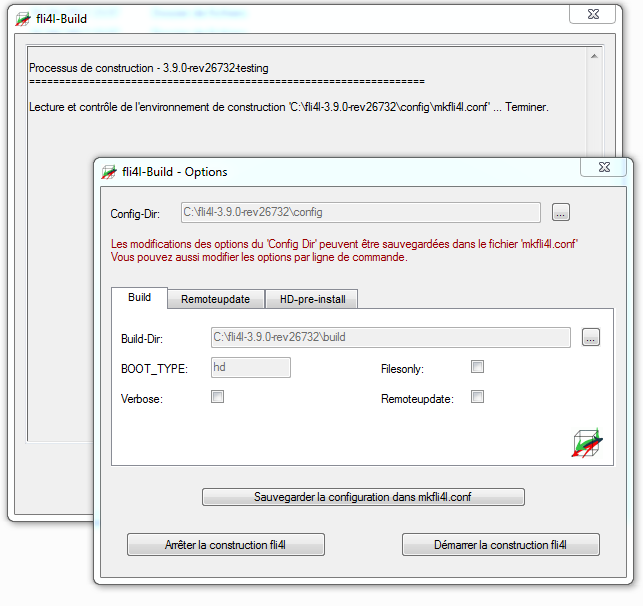
\includegraphics[width=\columnwidth]{win_build_build}
  \caption{Paramètre}
  \label{fig:win_build_build}
  \end{figure}

  On défini dans cette fenêtre, la sauvegarde des paramètres et la création du média~:
  \begin{itemize}
    \item Build-Dir~-- Répertoire pour l'archive/l'image CD/...
    \item \var{BOOT\_TYPE}~-- Régle l'affichage/utilisé \var{BOOT\_TYPE}~-- il ne peut pas être modifié ici
    \item Verbose~--- Affiche les informations pendant la construction du programme fli4l
    \item Filesonly~--- Sauvegarde uniquement les fichiers, pas de création d'image
    \item Remoteupdate~--- Active la mise à jour par SCP
  \end{itemize}

  Avec le bouton \textbf{les paramètres du programme fli4l-build peuvent être sauvegardés à tout moment},
       les paramètres seront enregistrés dans le fichier mkfli4l.txt, ils
       peuvent être modifié manuellement en ouvrant ce fichier.


  \subsection{Boîte de dialogue~-- Paramètres pour la mise à jour à distance}
  \begin{figure}[h!]
  \centering
  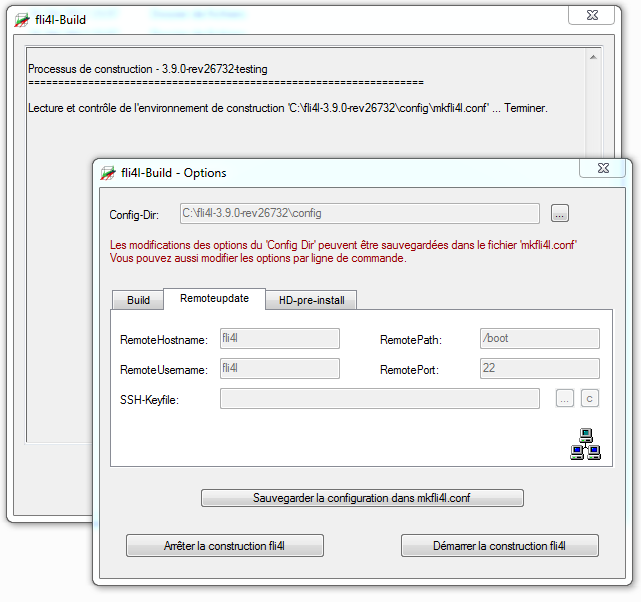
\includegraphics[width=\columnwidth]{win_build_remoteupdate}
  \caption{Paramètre pour la mise à jour}
  \label{fig:win_build_remoteupdate}
  \end{figure}

  On défini dans cette fenêtre, les réglages pour l'installation d'une mise à jour~:
  \begin{itemize}
    \item Adresse IP ou Nom d'Hôte
    \item Nom d'utilisateur sur l'hôte distant
    \item Remote-path (Par défaut: /boot)
    \item Remote-port (Port par défaut: 22)
    \item Utiliser SSH-Keyfile (Format ppk de Putty)
  \end{itemize}

  \subsection{Boîte de dialogue~-- Paramètres pour une pré-installation du HD}
  \begin{figure}[h!]
  \centering
  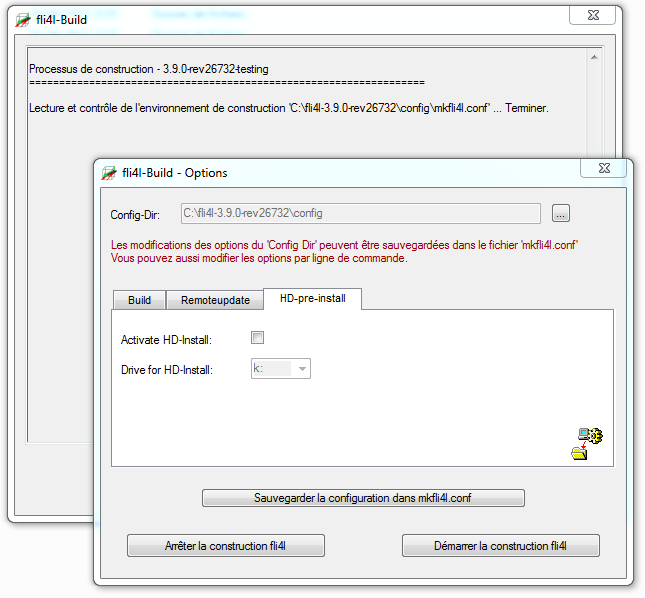
\includegraphics[width=\columnwidth]{win_build_hd_install}
  \caption{Paramètre pour pré-installation du DD}
  \label{fig:win_build_hd_install}
  \end{figure}

   On défini dans cette fenêtre, les paramètres pour la pré-installation
   d'un disque dur, une Carte CompactFlash, une clef USB formaté et partitionné.

   Options possibles~:
  \begin{itemize}
     \item Active la pré-installation du Disque Dur
     \item Lettre du lecteur ou de la Carte-CF
  \end{itemize}

  Information pour partitionner et formater CF (Compact Flash)~: Pour
  cette installation utiliser le TYPE A, de plus (nous avons besoin
  du paquetage HD), une partition FAT primaire doit être active et
  formatée sur la CF. Si l'on veut utiliser une partition bootable
  il faut installer une partition Linux supplémentaire formatée avec
  le système ext3, on aura besoin du fichier \texttt{hd.cfg} sur la partition
  FAT (pour cela il faut absolument installer et configurer le paquetage HD).


\marklabel{sec:mkfli4lconf}{
  \section{Paramètre pour le fichier mkfli4l.txt}}

  Il existe depuis la Version fli4l 2.1.9, le fichier de
  configuration \texttt{$<$config$>$/mkfli4l.txt}. Toutes les commandes
  du programme 'graphique' fli4l-Build sont enregistrées dans
  le fichier mkfli4l.txt. Le fichier est construit comme tous
  les fichiers fli4l. Toutes les variables de configuration sont
  optionnelles, mais il ne faut pas, modifier les variables spécifiques.

  \begin{description}

  \config {BUILDDIR}{BUILDDIR}{BUILDDIR}

  Valeur par défaut~: 'build'

  On indique ici le nom du répertoire pour enregistrer les fichiers de
  construction pour le boot de fli4l. Si la variable n'est pas définie, mkfli4l
  sous Windows utilisera par défaut le sous-répertoire \texttt{build} de la racine
  du répertoire fli4l~:
  \begin{verbatim}
     Chemin/fli4l-x.y.z/build
  \end{verbatim}
  \vspace{-2ex}
  En lancant mkfli4l le programme enregistre des fichiers de
  construction produits dans le répertoire \texttt{$<$config$>$/build}.

  Vous devez utiliser les conventions des systèmes d'exploitation de Windows ou
  *Unix pour paramétrer le chemin d'accès \var{BUILDDIR}. Si vous avez paramétré
  un chemin relatif, ce chemin sera converti par le processus de construction
  de Windows ou *Unix.

  \config {VERBOSE}{VERBOSE}{VERBOSE}

  Valeur par défaut~: \var{VERBOSE='no'}

  Valeurs possibles sont \var{'yes'} ou \var{'no'}. Affiche les
  \emph{les Informations} du processus Build (ou processus de construction).

  \config {FILESONLY}{FILESONLY}{FILESONLY}

  Valeur par défaut~: \var{FILESONLY='no'}

  Valeurs possibles \var{'yes'} ou \var{'no'}. Vous permet de créer un Boot
  média, peut être désactivé de sorte à créer uniquement les fichiers d'archives.

  \config {REMOTEUPDATE}{REMOTEUPDATE}{REMOTEUPDATE}

  Valeur par défaut~: \var{REMOTEUPDATE='no'}

  Valeurs possibles \var{'yes'} ou \var{'no'}. Si on veut transmettre
  automatiquement des fichiers de boot sur le Routeur au moyen de SCP.
  Cela suppose que le paquetage \jump{OPTSSHD}{SSHD} est installé et
  en plus la variable \texttt{scp} soit activée dans se paquetage.

  \config {REMOTEHOSTNAME}{REMOTEHOSTNAME}{REMOTEHOSTNAME}

  Valeur par défaut~: \var{REMOTEHOSTNAME=''}

  On indique ici le nom d'hôte du destinataire pour le transfert des
  données avec SCP. Si vous n'avez indiqué aucun nom, le nom de la
  variable \jump{HOSTNAME}{\var{HOSTNAME}} est utilisée pour le
  transfert des données.

  \config {REMOTEUSERNAME}{REMOTEUSERNAME}{REMOTEUSERNAME}

  Valeur par défaut~: \var{REMOTEUSERNAME='fli4l'}

  Nom d'utilisateur pour la transmission des données SCP.

  \config {REMOTEPATHNAME}{REMOTEPATHNAME}{REMOTEPATHNAME}

  Valeur par défaut~: \var{REMOTEPATHNAME='/boot'}

  Chemin d'accès du destinataire pour la transmission des données SCP.

  \config {REMOTEPORT}{REMOTEPORT}{REMOTEPORT}

  Valeur par défaut~: \var{REMOTEPORT='22'}

  Port du destinataire pour la transmission des données SCP.

  \config {SSHKEYFILE}{SSHKEYFILE}{SSHKEYFILE}

  Valeur par défaut~: \var{SSHKEYFILE=''}

  Ici on peut indiquer le fichier de clef-SSH pour la mise à jour
  avec SCP. Un mot de passe peut aussi être demandé pour la mise à jour.

  \config {REMOTEREMOUNT}{REMOTEREMOUNT}{REMOTEREMOUNT}

  Valeur par défaut~: \var{REMOTEREMOUNT='no'}

  Les valeurs possibles sont \var{'yes'} ou \var{'no'}. Si vous indiquez
  \var{'yes'}, vous remontez le boot device "/boot" en lecture/écriture
  si le boot est en lecture seule, c'est pour monter et rendre possible
  la mise à jour distante.

  \config {TFTPBOOTPATH}{TFTPBOOTPATH}{TFTPBOOTPATH}

  Le chemin d'accès pour installer l'image de boot par le réseau.

  \config {TFTPBOOTIMAGE}{TFTPBOOTIMAGE}{TFTPBOOTIMAGE}

  Nom de l'image de boot sur le réseau.

  \config {PXESUBDIR}{PXESUBDIR}{PXESUBDIR}

  Sous-répertoire pour les fichiers PXE qui est en rapport avec TFTPBOOTPATH.

  \config {SQUEEZE\_SCRIPTS}{SQUEEZE\_SCRIPTS}{SQUEEZESCRIPTS}

  Active ou désactive Squeeze (compression des scripts). Par ex. un
  Script qui contient en plus des lignes de commentaires, ces lignes
  serons supprimées à la compressé par Squeeze. Normalement on devrais
  toujours indiquer \var{'yes'} dans cette variable.

  \config {MKFLI4L\_DEBUG\_OPTION}{MKFLI4L\_DEBUG\_OPTION}{MKFLI4LDEBUGOPTION}

   Options supplémentaires de débugage, peut être transmis au \jump{mkfli4l}{Programme-mkfli4l}.

  \end{description}

  \chapter{Réglage des PCs dans le LAN}

  Réglage des ordinateurs dans le LAN (ou réseau local)~:

  \begin{enumerate}
  \item Adresse IP (voir \smalljump{sec:pc-lan-ip}{Adresse IP})
  \item Nom de l'ordinateur et Nom de Domaine
    (voir \smalljump{sec:pc-lan-name}{Nom de l'ordinateur et de Domaine})
  \item Gateway-Standard (Passerelle Standard) (voir \smalljump{sec:pc-lan-gateway}{Gateway})
  \item Adresse IP et serveur-DNS (voir \smalljump{sec:pc-lan-dns}{Serveur-DNS})
  \end{enumerate}


  \marklabel{sec:pc-lan-ip}{\section{Adresse IP}}
  Les adresses IP du réseau local doivent se trouver dans le même
  réseau que l'adresse IP du routeur fli4l (de l'interface Ethernet),
  par ex. 192.168.6.2 pour l'ordinateur local dans le cas ou le routeur
  aurait l'adresse IP 192.168.6.1. Les adresses IP doivent être uniques
  dans le réseau, changer uniquement le dernier chiffre de l'adresse IP
  est un bon moyen pour ne pas se tromper. Vous devez vous assurez que
  l'adresses IP indiqué ici est la même adresse IP que vous avez config
  pour cet ordinateur dans le fichier config/base.txt.

  \marklabel{sec:pc-lan-name}{\section{Nom de l'ordinateur et de domaine}}
  Le nom de l'ordinateur est par ex. "mon-pc", et le nom de Domaine "lan.fli4l".

  \wichtig{Le domaine qui est réglé dans le PC doit être identique
   au domaine choisi dans l'ordinateur fli4l, si on veut utiliser le
   routeur fli4l comme serveur DNS, il peut y avoir d'énormes problèmes
   dans le réseau si les domaines sont différents.}

  La raison~: les ordinateurs Windows cherchent régulièrement les
  ordinateurs avec le même nom de groupe de travail WORKGROUP.mon-domain.fli4l.
  Si fli4l ne répond pas à la requête du domaine (ici~: mon-domain.fli4l),
  alors fli4l essayera de chercher le domaine en se connectant sur Internet \ldots

  Le domaine doit être enregistré dans les réglages TCP/IP de l'ordinateur.

  \subsection{Windows 2000}

  Pour Windows 2000 se trouve sous~:

  \noindent Démarrer \pfeil\\
  \hspace*{2ex}Paramètre \pfeil\\
  \hspace*{4ex}Panneau de configuration \pfeil\\
  \hspace*{6ex}Connexion réseau \pfeil\\
  \hspace*{8ex}Connexion au réseau local \pfeil\\
  \hspace*{10ex}Bouton droit propriétés  \pfeil\\
  \hspace*{12ex}Protocole Internet (TCP/IP) \pfeil\\
  \hspace*{14ex}Sélectionner \pfeil\\
  \hspace*{16ex}Avancé \ldots \pfeil\\
  \hspace*{18ex}DNS \pfeil\\
  \hspace*{20ex}Suffix DNS pour cette connexion \pfeil\\

  Entrer "lan.fli4l" (ou indiquer votre domaine) (sans les "" !)
  \pfeil et appuyez sur OK.

\subsection{NT 4.0}

  Démarrer \pfeil\\
  \hspace*{2ex}Paramètre \pfeil\\
  \hspace*{4ex}Panneau de configuration  \pfeil\\
  \hspace*{6ex}Réseau \pfeil\\
  \hspace*{8ex}Protocole \pfeil\\
  \hspace*{10ex}TCP/IP \pfeil\\
  \hspace*{12ex}Propriétés \pfeil\\
  \hspace*{14ex}DNS \pfeil\\
  \hspace{16ex}\begin{itemize}
  \item Nom d'hôte entrer (le Nom de l'ordinateur)
  \item Domaine entrer (le même Nom que dans le fichier config/base.txt)
  \item Ajouter adresse IP le même réseau que le routeur fli4l
  \item Ajouter suffix DNS (Domaine le même que la ligne 2)
  \end{itemize}

\subsection{Windows 95/98}

  Démarrer \pfeil\\
  \hspace*{2ex}Paramètre \pfeil\\
  \hspace*{4ex}Panneau de configuration \pfeil\\
  \hspace*{6ex}Réseau \pfeil\\
  \hspace*{8ex}Configuration \pfeil\\
  \hspace*{10ex}TCP/IP (sélectionner la carte réseau qui va au routeur) \pfeil\\
  \hspace*{12ex}propriétés \pfeil\\
  \hspace*{14ex}Configuration DNS~:

  Cliquer activé DNS, dans le champ "Domaine"~: entrer "lan.fli4l"
  (ou indiquer votre domaine) (sans les "" !).

\subsection{Windows XP}

  Pour Windows XP se trouvent sous~:

  \noindent Démarrer \pfeil\\
  \hspace*{2ex}Paramètre \pfeil\\
  \hspace*{4ex}Panneau de configuration \pfeil\\
  \hspace*{6ex}Connexions réseau \pfeil\\
  \hspace*{8ex}Connexion au réseau local \pfeil\\
  \hspace*{10ex}Propriétés \pfeil\\
  \hspace*{12ex}Protocole Internet (TCP/IP) \pfeil\\
  \hspace*{14ex}Propriétés \pfeil\\
  \hspace*{16ex}Avancé\ldots \pfeil\\
  \hspace*{18ex}DNS \pfeil\\
  \hspace*{20ex}Suffixe DNS pour cette connexion \pfeil\\

  Indiquez "lan.fli4l" (ou indiquer votre domaine) (sans les "" !)
  \pfeil Cliquez sur OK.

  \subsection{Windows 7}

  Pour Windows 7 se trouvent sous~:

  \noindent Bouton Windows (ex. Démarrer) \pfeil\\
  \hspace*{2ex}Contrôle \pfeil\\
  \hspace*{4ex}Panneau de configuration \pfeil\\
  \hspace*{6ex}Centre Réseau et partage \pfeil\\
  \hspace*{8ex}Connexion au réseau local \pfeil\\
  \hspace*{10ex}Propriétés \pfeil\\
  \hspace*{12ex}Protocole Internet version 4 (TCP/IPv4) \pfeil\\
  \hspace*{14ex}Propriétés \pfeil\\
  \hspace*{16ex}Avancé\ldots \pfeil\\
  \hspace*{18ex}DNS \pfeil\\
  \hspace*{20ex}Suffixe DNS pour cette connexion \pfeil\\

  Indiquez "lan.fli4l" (ou indiquer votre domaine) (sans les "" !)
  \pfeil Cliquez sur OK.

\subsection{Windows 8}

  Pour Windows 8 se trouvent sous~:

  \noindent Appuyez simultanément sur la touche Windows et X \pfeil\\
  \hspace*{2ex}Contrôle \pfeil\\
  \hspace*{4ex}Connexions réseau \pfeil\\
  \hspace*{6ex}Sélectionnez votre réseau (Ehternet ou WLAN) \pfeil\\
  \hspace*{8ex}Clique droit \pfeil\\
  \hspace*{10ex}Propriétés \pfeil\\
  \hspace*{12ex}Protocole Internet version 4 (TCP/IPv4) \pfeil\\
  \hspace*{14ex}Propriétés \pfeil\\
  \hspace*{16ex}Avancé\ldots \pfeil\\
  \hspace*{18ex}DNS \pfeil\\
  \hspace*{20ex}Suffixe DNS pour cette connexion \pfeil\\

  Indiquez "lan.fli4l" (ou indiquer votre domaine) (sans les "" !)
  \pfeil Cliquez sur OK.

  \marklabel{sec:pc-lan-gateway}{\section{Gateway (ou Passerelle)}}

  Il est absolument nécessaire d'indiquer une adresse IP dans le paramètre
  passerelle par défaut de votre PC, car s'il n'y a pas d'adresse IP d'indiquée,
  rien ne fonctionnera. Ainsi vous devrez indiquer l'adresse IP du routeur
  fli4l - (Interface Ethernet) par exemple 192.168.6.4, selon l'adresse
  IP qui est configurée dans le fichier config/base.txt du routeur fli4l.

  Il est incorrect de configuter le routeur fli4l comme un proxy dans Windows
  ou dans de votre navigateur~-- sauf si vous définissez un proxy sur votre
  routeur fli4l. Normalement fli4l a pas de proxy, s'il vous plaît ne spécifiez
  \emph{pas} fli4l comme un proxy~!

\marklabel{sec:pc-lan-dns}{\section{Serveur DNS}}

  Pour l'adresse IP du serveur DNS, vous ne devez pas indiquer
  d'adresse IP de votre fournisseur d'accés Internet mais l'adresse IP
  du routeur (interface Ethernet), car le routeur peut répondre aux
  requêtes DNS et faire suivre ceux-ci par Internet si nécessaire.

  Quand fli4l est utilisé comme serveur DNS, beaucoup de requêtes
  DNS son envoyées par les PCs client Windows, c'est le routeur fli4l qui
  leur répond directement, elles ne sont pas expédiées sur Internet.

\marklabel{sec:pc-lan-misc}{\section{Divers points }}

  Les points 1 et 4 n'ont pas besoin d'être enregistrés avec un
  serveur DHCP puisque le routeur fli4l communique les données
  nécessaires automatiquement.

  \textbf{Dans Options Internet~:} et dans la fenètre connexion vous ne devez
  "sélectionner aucun lien". Dans Paramètre réseau local (LAN)~: ne RIEN
  indiquer (sauf si vous utilisez le paquetage \var{OPT\_\-P}roxy).
  Par défaut les deux paramètres n'ont pas besoin d'être modifié pour
  une utilisation normale.


  \marklabel{IMONDSCHNITTSTELLE}{
    \chapter{Interface client/serveur imon}
  }

  \marklabel{sec:imond}{
    \section{Server imon avec imond}}

  Imond est un programme serveur qui répond à certaines enquêtes sur
  la gestion du réseau et accepte aussi des commandes qui peuvent contrôler
  le routeur sur le réseau local.

  Imond contrôle également les Moindres-Coûts-Routages. Il utilise
  le fichier de configuration /etc/imond.conf qui est produit
  automatiquement au moment du boot, à partir de la variable \var{ISDN\_\-CIRC\_\-x\_\-XXX}
  du fichier config/isdn.txt, le fichier est généré par un script shell.

  imond est un démon qui fonctionne en permanence en tache de fond,
  il écoute le port 5000 TCP/IP sur le périphérique /dev/isdninfo.

  Voici toutes les commandes qui peuvent être envoyées par le port 5000 TCP/IP~:
  \begin{table}
    \textbf{Commandes Admin}

    \vspace{1ex}
    \begin{tabular}{lp{9cm}}

      addlink ci-index              & Ajouter un canal au circuit (Channel-Bundling) \\
      adjust-time seconds           & Incrémente la date sur le routeur en secondes \\
      delete filename pw            & Supprime le fichier sur le routeur \\
      hup-timeout \#ci-index [value]& Affiche ou compose le HUP-Timeout pour
                                      des circuits RNIS (ou numéris) \\
      removelink ci-index           & Enlever le canal supplémentaire \\
      reset-telmond-log-file        & Supprime le fichier journal de telmond \\
      reset-imond-log-file          & Supprime le fichier journal de imond \\
      receive filename \#octets pw  & Transfére d'un fichier au routeur.
                                      Imond donne l'ordre avec ACK (0x06). Après,
                                      le fichier est transféré par blocs de 1024
                                      Octets qui sont également confirmé avec ACK.
                                      En conclusion, imond répond OK. \\
      send filename pw              & Si le mot de passe est correct et que le
                                      fichier existe, imond répond OK avec un \#octet.
                                      Puis, imond transfère le fichier par blocs de
                                      1024 octets, chaque fois confirmés avec ACK
                                      (0x06). A la fin, imond répond OK. \\
      support pw                    & Montre le statut/configuration du routeur \\
      sync                          & Synchronise le Cache des lecteurs montés \\
    \end{tabular}
  \end{table}


  \begin{table}
    \textbf{Commandes Admin et Utilisateur}

    \vspace{1ex}
    \begin{tabular}{lp{9cm}}

      dial                      &    Choix du FAI (Defaut-Route-Circuit) \\
      dialmode [auto|manual|off]&    Réglage des actions dans Dialmode \\
      disable                   &    Raccroche et place dialmode sur "off" \\
      enable                    &    Mets dialmode sur "auto" \\
      halt                      &    Descend proprement le Routeur \\
      hangup [\#channel-id]     &    Raccroche \\
      poweroff                  &    Descent le routeur et mise hors tension \\
      reboot                    &    Reboot le routeur fli4l! \\
      route [ci-index]          &    Met le routeur par Defaut sur un Circuit X (0=automatique) \\
    \end{tabular}
  \end{table}


  \begin{table}
    \textbf{Commandes Utilisateur}

    \vspace{1ex}
    \begin{tabular}{lp{9cm}}
      channels                  & Nombre de Canaux ISDN disponibles \\
      charge \#channel-id       & Edite les frais de connexion pour un Canal en ligne \\
      chargetime \#channel-id   & Temps et frais de connexion pour un canal en ligne \\
      circuit [ci-index]        & Edite le numéro du Circuit \\
      circuits                  & Edite le nombre de Defaut-Route-Circuits \\
      cpu                       & Donne la charge du CPU en pourcentage \\
      date                      & Edite la date et heure \\
      device ci-index           & Circuits du périphérique utilisé \\
      driverid \#channel-id     & Edite Driver-ID pour le Canal X \\
      help                      & Edite l'aide \\
      inout \#channel-id        & Edite la direction (entrante/sortante) \\
      imond-log-file            & Edite le fichier du Protocole imond \\
      ip \#channel-id           & Edite l'adresse IP \\
      is-allowed command        & Edite si la commande est valide\newline
                                  commandes possibles~:
                                  dial|dialmode|route|reboot
                                  |imond-log|telmond-log|mgetty-log \\
      is-enabled                & Edite si dialmode est sur off (0) ou auto (1) \\
      links ci-index            & Edite le nombre de canaux 0, 1 ou 2, 0 utilisé,
                                  ou alors~: Aucun Channel-Bundling possible \\
      log-dir imond|telmond|mgetty& Donne la direction des fichiers Log \\
      mgetty-log-file           & Edite le protocole du fichier mgetty \\
      online-time \#channel-id  & Edite le temps en ligne, et de connexion en hh:mm:ss \\
      pass [password]           & Vérifie, le mot de passe qui a été saisit par\newline
                                  1 Mot de passe Utilisateur est fixé\newline
                                  2 Mot de passe Admin est fixé\newline
                                  4 imond se trouve dans le mode Admin \\
      phone \#channel-id        & Edite le numéro de Tél et le nom du "correspondant" \\
      pppoe                     & Donne le numéro du périphérique pppoe (0 ou 1) \\
      quantity \#channel-id     & Donne l'ensemble des transmissions (en octet) \\
      quit                      & Coupe la connexion avec imond \\
      rate \#channel-id         & Edite les connexions (entrant/sortant en Octet/sec) \\
      status \#channel-id       & Edite le statut pour le Canal X \\
      telmond-log-file          & Edite le protocole telmond \\
      time \#channel-id         & Edite le temps total en ligne, au Format hh:mm:ss \\
      timetable [ci-index]      & Edite la time-table LC-Routing \\
      uptime                    & Edite le temps d'utilisation du Routeur en secondes \\
      usage \#channel-id        & Edite les réponses des connexions: Fax, Répondeur, Net, Modem, Raw \\
      version                   & Edite la version du protocole et la version du Programme \\
    \end{tabular}
  \end{table}


  Le port 5000 TCP/IP est accessible uniquement depuis un réseau LAN
  masqué. Avec la configuration standard du firewall l'accés est bloqué
  de l'extérieur.

  Imond supporte deux modes d'administrations, le Mode Utilisateur et
  le Mode Admin. On peut installer un Mot de Passe pour ces deux modes
  au moyen des variables \var{IMOND\_\-PASS} et \var{IMOND\_ADMIN\_\-PASS}.
  Si le Mot de Passe n'est pas transmis au serveur imond le client imonc
  a accés uniquement à deux commandes "pass" et "quit" toutes les autres
  commandes sont rejetées et une erreur s'affiche.

  Si plus tard, vous voulez limiter l'accés au serveur imond à un seul PC,
  la configuration du Firewall doit être modifier.

  Les commandes

\begin{example}
\begin{verbatim}
         enable/disable/dialmode   dial/hangup   route   reboot/halt
\end{verbatim}
\end{example}

  peuvent être activées ou désactivées dans la variable
  \var{IMOND\_\-XXX} voir (le chapitre "configuration").

  Avec un ordinateur Unix/Linux (ou un ordinateur Windows par la
  fenètre DOS) vous pouvez facilement entrer les commandes aprés
  la connexion telnet.

  Connexion telnet~:

\begin{example}
\begin{verbatim}
        telnet fli4l 5000        \# ou le Nom correspondant au routeur fli4l
\end{verbatim}
\end{example}

  Vous pouvez directement entrer les commandes mentionnées ci-dessus.

  Par exemple la commande "help" active l'aide sur l'écran ou "quit"
  démonte (ou arrête) le serveur imond.

\marklabel{sec:leastcostrouting}{
  \subsection{Mode de fonctionnement du Moindre-Coût-Routage}
  }

  imond construit une Time-Table (ou Plage Horaire) à partir du fichier
  de configuration /etc/imond.conf (qui est créé au boot avec la variable
  de configuration \var{ISDN\_\-CIRC\_\-x\_\-TIMES}. Ce "calendrier" est
  composé d'une semaine par intervalle d'une heure, une semaine = 168
  heures = 168 octets. La table se compose de circuits, dans lesquel sont
  définis des Défaut-Routes (ou connexion par défaut au FAI).

  Avec la commandement "timetable" on peut voir la table imond.
  Exemple de configuration~:

Supposons que nous définissions 3 circuits de connexions pour chaque FAI c'est à dire~:

\begin{example}
\begin{verbatim}
        CIRCUIT_1_NAME='Addcom'
        CIRCUIT_2_NAME='AOL'
        CIRCUIT_3_NAME='Firma'
\end{verbatim}
\end{example}

  Les deux premiers circuits sont réglés avec Défaut-Route c.à d.
  que l'itinétaire par défaut est écrit dans la variable
  ISDN\_CIRC\_x\_ROUTE avec la valeur '0.0.0.0/0'.

  Les variables \var{ISDN\_\-CIRC\_\-x\_\-TIMES} se présentent de la manière suivante~:

\begin{example}
\begin{verbatim}
        ISDN_CIRC_1_TIMES='Mo-Fr:09-18:0.0388:N Mo-Fr:18-09:0.0248:Y
                      Sa-Su:00-24:0.0248:Y'

        ISDN_CIRC_2_TIMES='Mo-Fr:09-18:0.019:Y Mo-Fr:18-09:0.049:N
                      Sa-Su:09-18:0.019:N Sa-Su:18-09:0.049:N'

        ISDN_CIRC_3_TIMES='Mo-Fr:09-18:0.08:N Mo-Fr:18-09:0.03:N
                      Sa-Su:00-24:0.03:N'
\end{verbatim}
\end{example}

  Puis le fichier /etc/imond.conf est créé de cette façon~:

\begin{example}
\begin{verbatim}
        #day  hour  device  defroute  phone        name        charge  ch-int
        Mo-Fr 09-18 ippp0   no        010280192306 Addcom      0.0388   60
        Mo-Fr 18-09 ippp0   yes       010280192306 Addcom      0.0248   60
        Sa-Su 00-24 ippp0   yes       010280192306 Addcom      0.0248   60
        Mo-Fr 09-18 ippp1   yes       019160       AOL         0.019   180
        Mo-Fr 18-09 ippp1   no        019160       AOL         0.049   180
        Sa-Su 09-18 ippp1   no        019160       AOL         0.019   180
        Sa-Su 18-09 ippp1   no        019160       AOL         0.049   180
        Mo-Fr 09-18 isdn2   no        0221xxxxxxx  Firma       0.08     90
        Mo-Fr 18-09 isdn2   no        0221xxxxxxx  Firma       0.03     90
        Sa-Su 00-24 isdn2   no        0221xxxxxxx  Firma       0.03     90
\end{verbatim}
\end{example}

  imond produit alors Time-Table (ou Plage Horaire) dans la mémoire.
  voici la table des données sorties avec la commande "timetable"~:

\begin{example}
\begin{verbatim}
         0  1  2  3  4  5  6  7  8  9 10 11 12 13 14 15 16 17 18 19 20 21 22 23
     --------------------------------------------------------------------------
     Su  3  3  3  3  3  3  3  3  3  3  3  3  3  3  3  3  3  3  3  3  3  3  3  3
     Mo  2  2  2  2  2  2  2  2  2  4  4  4  4  4  4  4  4  4  2  2  2  2  2  2
     Tu  2  2  2  2  2  2  2  2  2  4  4  4  4  4  4  4  4  4  2  2  2  2  2  2
     We  2  2  2  2  2  2  2  2  2  4  4  4  4  4  4  4  4  4  2  2  2  2  2  2
     Th  2  2  2  2  2  2  2  2  2  4  4  4  4  4  4  4  4  4  2  2  2  2  2  2
     Fr  2  2  2  2  2  2  2  2  2  4  4  4  4  4  4  4  4  4  2  2  2  2  2  2
     Sa  3  3  3  3  3  3  3  3  3  3  3  3  3  3  3  3  3  3  3  3  3  3  3  3

     No.  Name                   DefRoute  Device  Ch/Min   ChInt
      1   Addcom                   no      ippp0   0.0388     60
      2   Addcom                   yes     ippp0   0.0248     60
      3   Addcom                   yes     ippp0   0.0248     60
      4   AOL                      yes     ippp1   0.0190    180
      5   AOL                      no      ippp1   0.0490    180
      6   AOL                      no      ippp1   0.0190    180
      7   AOL                      no      ippp1   0.0490    180
      8   Firma                    no      isdn2   0.0800     90
      9   Firma                    no      isdn2   0.0300     90
     10   Firma                    no      isdn2   0.0300     90
\end{verbatim}
\end{example}

  Pour le circuit 1 (Addcom) il y a trois éléments définis (1-3),
  pour le circuit 2 il y a quatre éléments (4-7), et pour le circuit 3
  il y a trois éléments (8-10).

  Les index des circuits activés sont inscris toutes les heures dans
  la Time-Table respectivement. Ici les index (2-4) apparaissent,
  car les autres ne passent pas par LC-Défaut-Route.

  Si vous avez des zéros dans Time-Table, c'est qu'il manque des données
  dans la variable \var{ISDN\_\-CIRC\_\-X\_\-TIMES}. Si vous avez des
  zéro sur certaine plage horaire, cela veux dire qu'il n'y aura pas de
  Défaut-Route et aucun accés Internet possible sur ces plages horaires!

  Au démarrage du programme, imond vérifie le jour de la semaine et
  l'heure, puis les index dans la Time-Table et enfin régle les Défauts-Routes
  correspondants. Le Défaut-Route (ou connexion par Défaut au FAI) est alors
  activé par rapport à l'indexation.

  Lors d'un changement de statut, par exemple sur un canal, une connexion
  ou un racrochement de la ligne, si la commande mais plus d'une minute,
  le processus de démarrage est réactualisé, vérification de l'horaire et
  du jour, consultation de la table, selection du Circuit-Défaut-route.

  Si par exemple le lundi à 18:00 la connexion change, Défaut-Route est
  supprimé, les connexions existantes sont arrêtées (désolé\ldots),
  ensuite imond controle dans la Time-Table si un nouveau Circuit-Défaut-route
  existe, si oui imond mettra environ 60 secondes pour se reconnecter.
  Donc la connexion se fera au plus tard à 18:00:59.

  Il n'y aura aucun changement pour les circuits qui n'utilisent pas
  un Defaut-Route. Le contenu \var{ISDN\_\-CIRC\_\-x\_\-TIMES} sera
  uniquement employé pour le calcul des frais téléphoniques. Ceci peut
  être pertinent, si vous arrêtez temporairement le client imonc et que
  vous choisissiez manuellement un Circuit-Défaut-route.

  Vous pouvez également regarder dans l'indexation de Time-Table (exemple
  précédent de 1 à 10) les circuits non activés "Non-LC-Default-Route-Circuits".

  Commande pour vérifier un index dans le Time-Table~:

\begin{example}
\begin{verbatim}
                    timetable "index"
\end{verbatim}
\end{example}

  Exemple~:

\begin{example}
\begin{verbatim}
                    telnet fli4l 5000
                    timetable 5
                    quit
\end{verbatim}
\end{example}

  La sortie des données apparaîtront comme ceci~:

\begin{example}
\begin{verbatim}
         0  1  2  3  4  5  6  7  8  9 10 11 12 13 14 15 16 17 18 19 20 21 22 23
     --------------------------------------------------------------------------
     Su  0  0  0  0  0  0  0  0  0  0  0  0  0  0  0  0  0  0  0  0  0  0  0  0
     Mo  5  5  5  5  5  5  5  5  5  0  0  0  0  0  0  0  0  0  5  5  5  5  5  5
     Tu  5  5  5  5  5  5  5  5  5  0  0  0  0  0  0  0  0  0  5  5  5  5  5  5
     We  5  5  5  5  5  5  5  5  5  0  0  0  0  0  0  0  0  0  5  5  5  5  5  5
     Th  5  5  5  5  5  5  5  5  5  0  0  0  0  0  0  0  0  0  5  5  5  5  5  5
     Fr  5  5  5  5  5  5  5  5  5  0  0  0  0  0  0  0  0  0  5  5  5  5  5  5
     Sa  0  0  0  0  0  0  0  0  0  0  0  0  0  0  0  0  0  0  0  0  0  0  0  0

     No.  Name                   DefRoute  Device  Ch/Min   ChInt
      5   AOL                      no      ippp1   0.0490    180
\end{verbatim}
\end{example}

  Tout est clair jusque là~?

  Avec la commande "Route" d'imond vous pouvez commuter "Marche/Arrêt"
  de LC-Routing, et vous pouvez indiquer l'index du Circuit-Défaut-Route
  (1\ldots N), il se connectera sur le circuit. Si l'index est 0, le
  LC-Routing est activé et le circuit sera choisi automatiquement.

  \subsection{Calcul des frais on-line (en ligne)}

  Le mode de calcul des frais de connexions fonctionnera correctement
  uniquement si l'unité téléphonique est constante tout au long
  de la semaine, elle doit est inscrit dans la variable
  \var{ISDN\_\-CIRC\_\-x\_\-CHARGEINT}) en seconde. Normalement c'est la
  régle pour les fournisseurs d'accés Internets. Toutefois, si vous choisissez
  Telekom (je ne parle pas de T-Online~!) par exemple, pour un réseau
  d'entreprise, qui sera considéré comme des conversations téléphoniques normales.
  et changement passe de 90 secondes à 4 minutes aprés 18:00 (Stand Juni
  00). Par conséquent, la définition

   Mais si vous utilisez votre
  société téléphonique par exemple pour un accés Internet avec TéléKom
  (Allemagne) l'unité Tél change (information juin 2000).\\
  En France l'unité Tél est toujours constante 60 secondes, on n'a
  pas ce problème, c'est juste le tarif qui change en heure creuse
  0,018 euro et en heure pleine 0,033 euro (8:00 à 19:00 heure pleine).

\begin{example}
\begin{verbatim}
        ISDN_CIRC_3_CHARGEINT='90'
        ISDN_CIRC_3_TIMES='Mo-Fr:09-18:0.08:N Mo-Fr:18-09:0.03:N Sa-Su:00-24:0.03:N'
\end{verbatim}
\end{example}

  est en fait pas tout à fait exact. Le tarif le soir est de 3 cents la minute
  (donc 12 cents les 4 minutes de télécommunication), mais la mesure est fausse.
  C'est pour cette raison qu'il se produit des différences d'affichage par
  rapport au prix réel.

  Il est possible que ce problème soit peut être corrigé plus tard.
  En attendant on peut définir dans la variable \var{ISDN\_\-CIRC\_\-x\_\-CHARGEINT})
  2 Circuits~: un pour la journée avec \var{ISDN\_\-CIRC\_\-1\_\-CHARGEINT}='90'
  et l'autre pour la soirée \var{ISDN\_\-CIRC\_\-2\_\-CHARGEINT}='240'
  naturellement vous devez configurer \var{ISDN\_\-CIRC\_\-x\_\-TIMES},
  avec cette configuration vous utiliser le Circuit 1 pendant la journée
  et le Circuit 2 en soirée.

  Comme nous l'avons dit plus haut~: l'utilisation des connexions avec
  un fournisseur d'accés Internet, ne pose pas de problème parce que
  l'unité Tél est toujours constante et le coût par minute ne change pas
  (il a encore quelque chose? je ne fais pas confiance à T-* pour tout :-).


  % Synchronized to r30003
  \marklabel{sec:winimonc}{
    \section{Windows-Client imonc.exe}}

  \subsection{Introduction}

  imond on the router and on the client imonc as a team have
  two use modes: the user and the admin mode. In admin mode, all
  controls are enabled. In user mode the variables
  \jump{IMONDENABLE}{\var{IMOND\_ENABLE}}, \jump{IMONDDIAL}{\var{IMOND\_DIAL}}, 
  \jump{IMONDROUTE}{\var{IMOND\_ROUTE}} and \jump{IMONDREBOOT}{\var{IMOND\_REBOOT}}
  control if the respective functions are available. If all of these
  variables are set to `no ', this means that all buttons in the overview page
  are disabled except for the exit and the admin mode button. The
  decision whether the user or admin mode is used, is based on the
  transmitted password. By clicking the button admin mode, located in the
  status bar, you may switch to the admin mode at any time by entering the
  admin password. To switch back imonc must be restarted.

  Once imonc is started an additional tray icon is displayed, which
  shows the connection status of existing channels.

  The colors mean:
  \begin{description}
    \item[Red]: Offline
    \item[Yellow]: A connection is in the process of being established
    \item[Light Green]: Online and traffic on the channel
    \item[Dark Green]: Online and (nearly) no traffic on the channel
  \end{description}

  \noindent imonc shows a behavior a little different from the Windows standard
  when clicking on the minimize button in the title bar. This minimizes imonc
  to the system tray only a tray icon near the clock remains. Double clicking
  on the tray icon with the left mouse button brings imonc's window back to
  the foreground. With the right mouse button you may use the context menu,
  of the tray icon to execute the main imonc commands die angezeigten
         without displaying its
  main window.

  Imonc stores many properties (including all columns widths of the string grids)
  in the registry, so its appearance may be widely adapted to your needs. Imonc
  uses the registry key HKCU{\textbackslash}Software{\textbackslash}fli4l
  to store this informations

  If even after careful reading of the documentation problems on imonc or the
  router itself still remain you can post to the newsgroup. It makes sense
  to note the support information you get when choosing SystemInfo and then Info
  on the About page of the imonc client. The router password will be queried
  then (not the imond password) and after that imonc will create a file fli4lsup.txt
  that contains all the important information regarding the router, including
  imonc. This file can be posted on the newsgroup when explicitely demanded
  and will give much better chance for quick help.

  Further details concerning the development of the Windows imonc client can be found
  on the homepage of Windows Imonc \altlink{http://www.imonc.de/}. Here you can
  see what new features and bug fixes will be included in the next version.
  In addition, you will find the latest imonc version, if it is not included
  in the FLI4L distribution already.

  \subsection{Start Parameters}

  Imonc requires the name or IP address of the router fli4l. As the default
  the program attempts to establish a connection with the computer ``fli4l''.
  If this entry is correctly entered in the DNS, this should work out of the box.
  Otherwise you can pass following parameters in the link:

  \begin{itemize}
    \item /Server:The router's IP or hostname (short form: /S:IP or hostname)
    \item /Password:password (short form: /P:password)
    \item /log Option for logging communication betweeen imonc und imond. When
      entered a file imonc.log  will be written each time when imonc exits. It
      contains the complete communication and thus can grow quite large. Please
      use this parameter only in case of problems.
    \item /iport:Portnumber Portnumber imond listens to. Default: 5000
    \item /tport:Portnummer Portnumber telmond listens to. Default: 5001
    \item /rc:''Command'' The command provided here will be transmitted to the
      router without further checking and imonc will exit afterwards. 
      If more than one command should be transmitted at once, they must be devided
      by semicolons. You will have to provide an imond password in addition for
      this to work because no password query will be queried. Possible command
      are documented with imond, see chapter 8.1. In addition to the commands
      there another one exists: timesync. If used imonc will synchronize the
      clock of the client with the router's clock. The command dialtimesync is
      not supported anymore, it is substituted by "dial; timesync".
    \item /d:''fli4l-Directory'' Pass the fli4l-directory as a start parameter.
      May be of interest when using more than one fli4l version.
    \item /wait If the hostname can't be reolved imonc will not exit anymore~--
      start another try by doubleclicking the tray icon.
    \item /nostartcheck Disables checking of imonc already running. Only makes
      sense to monitor several different fli4l routers in a net. When using more
      instances the builtin syslog- and \mbox{E-Mail}-capabilites will be disabled.
  \end{itemize}

  Usage (to be entered in the link):

\begin{example}
\begin{verbatim}
X:\...imonc.exe [/Server:Host] [/Password:Password] [/iport:Portnumber]
            [/log] [/tport:Portnumber] [/rc:"Command"]
\end{verbatim}
\end{example}

  Example with IP address:

\begin{example}
\begin{verbatim}
        C:\wintools\imonc /Server:192.168.6.4
\end{verbatim}
\end{example}

  or with name and password:

\begin{example}
\begin{verbatim}
        C:\wintools\imonc /S:fli4l /P:secret
\end{verbatim}
\end{example}

  or with name and password and router command:

\begin{example}
\begin{verbatim}
        C:\wintools\imonc /S:fli4l /P:secret /rc:"dialmode manual"
\end{verbatim}
\end{example}

  \subsection{Overview}

  The Windows client queries some imond information on the existing
  connections and displays it in its window. In addition to general
  status information such as uptime of the router or the time (both locally
  and on the router), for each existing connection the following informations
  are shown:

  \begin{tabular}{lp{9cm}}
    Status             &Connection establishment/Online/Offline\\
    Name               &Telephone number of the caller or circuit name\\
    Direction          &Indicates if a connection is incoming or outgoing\\
    IP                 &IP, that was assigned to the router\\
    IBytes             &Bytes received\\
    OBytes             &Bytes sent\\
    Online time        &Actual online time\\
    Time               &Sum of all online times\\
    KTime              &Sum of all online times in consideration of charge intervals\\
    Cost               &Computed costs\\
  \end{tabular}

  \medskip

  The data is updated every 2 seconds by default. In the context menu of
  this overview it is possible to copy the assigned IP to the clipboard
  as well as hanging up the channel (for each available channel which is
  online at the moment). This is of interest in case that several different
  connections exist, e.g. one to surf the Internet and another to a private
  net and only one of them should be terminated.

  If the telmond process is active on the router, imonc can show information
  about incoming phone calls (ie calling and called MSN) in addition. The last
  incoming phone call is displayed above the buttons. a log of phone calls received
  can be obtained by viewing the calls page.

  By the six buttons in imonc the following commands can be selected:

  \begin{tabular}{clp{9cm}}
    Button & Caption & Function \\
    1& Connect/Disconnect &   Dial/Hang up\\
    2& Add link/Rem link  &   Bundle channels: yes/no~-- only available in admin mode\\
    3& Reboot             &   Reboot fli4l!\\
    4& PowerOff           & Shut down fli4l and power off afterwards\\
    5& Halt               & Shut down fli4l to power off safe afterwards\\
    6& Exit               & Exit client\\
  \end{tabular}

  \medskip

  \noindent The first five commands can be switched on and off individually in the
  router's configuration file config/base.txt for the user mode. In admin mode all
  are enabled. The dialmode controls the dialing behavior of the router:

  \begin{tabular}{lp{9cm}}
    Auto  & The router will establish connections automatically when getting 
    queries from the local net for the circuit concerned.\\
    Manual & The user himself has to establish connections.\\
    Off   & No connections can be established. The dial button is deactivated.\\
  \end{tabular}

  \medskip

  \noindent Note that fli4l by default will dial out independently. So you never
  actually will have to press the connect button\ldots

  It is also possible to manually switch the default route circuit, setting
  the automatic LCR on and off. In the Windows version of imonc the selection
  list `` default route'' is provided for this. In addition you can configure the
  hangup TimeOut time directly in imonc. use the Config button next to the default
  route for this. All configured circuits of the router are displayed here. The
  value in the column Hup-timeout can be edited directly in the string grid
  for ISDN circuits (not yet working for DSL).

  An overview over LCR can be found on the page admin/Timetable.
  There you'll see what circuit imond selects automatically at which time.

  \subsection{Config-Dialog}

  The configuration is reached using the Config button in the status bar. The window
  is divided into the following areas:

  \begin{itemize}
  \item The Area General:
    \begin{itemize}
    \item Actualization Interval: Set here how often the overview should get actualized.
    \item Synchronize Time on Startup: When starting the client's system time and date 
      will get synchronized with the router's system time. You can execute this manually
      by using the button Synchronize on the Overview-page.
    \item Start Minimized: Program will start minimized to the system tray.
    \item Start with Windows: Specify here if the client should start automatically 
      with system start. Provide necessary start-parameters in the field Parameter.
    \item Fetch News from fli4l.de: Should news from fli4l's homepage be fetched and
      displayed by imonc? Then headlines are shown in the status bar. A new page News
      is displayed to show the complete messages.
    \item Logfile for Connections: The file name here is used to save connection lists
      locally on the imonc's system.
    \item TimeOut for router to answer: How long should we wait for an answer from the
      router before assuming that the connection has failed.
    \item Language: Pick the language for imoncs to use.
    \item Confirm Router Commands: If activated all commands influencing the router
      generally have to be confirmed, i.e. Reboot, Hangup \ldots
    \item Hang up even when traffic: No information should be displayed when the
      connection is closed and there is still traffic on the line.
    \item Automatic Connection to the router: Should we try to reconnect to the router
      in case of lost connections (i.e. when rebooting the router).
    \item Minimize Window To System Tray: Should imonc minimize to system tray instead
      of terminating itself when clicking the Exit button.
    \end{itemize}

  \item Proxy Settings:
    Define a proxy for imonc's http-queries here. It will be used for fetching news.
    \begin{itemize}
    \item Activate Proxy-support for Http-queries: Should we use a proxy 
          \begin{itemize}
            \item Address: Address of the proxy server
            \item Port: Port number of the proxy server (default: 8080)
          \end{itemize}
    \end{itemize}
    
  \item TrayIcon:
  	Set the colors of the tray icon next to the clock to your own needs.
  	In addition you can specify that the actual dialmode will set the background
  	color of the tray icon.

  \item Calls: The position of the call notification window will be saved in the
    registry in order to allow to set a fixed position for the window. Simlpy drag the
    window to the desired position.
    \begin{itemize}
      \item Update: Set here in what way imonc will be informed about new calls. There
	are three possibilities. The first is querying the telmond service on the
	router in regular time intervals. A second is evaluating the syslog messages.
	This variant is preferred to the first~- of course, the imon's syslog client
	has to be enabled. If imonc is used with a routed eisfair system the third
	possibility is to use the Capi2Text package for call signaling.
      \item Delete Leading Zeros (Phone Boxes): Phone boxes often use an additional
	Zero to prefix the caller's number. This option will suppress the digit.
      \item Own Area Code: Save your own area code here. If a call with the same
	area code is received it will get suppressed when displaying.
      \item Telephone Book: Here, the file can be specified, in which the local
        Phone book is saved for resolving of the phone number. If the file does not
        exist, it is created by the program.
      \item Logfile: The file name you can specify here is used to save the call
	list locally on the computer. This menu item is only visible if the config
	variable \var{TELMOND\_\-LOG} is set to `yes' (this also applies to the
        call list).
      \item Use External Search: In this area, a program may be specified that will
	be called when a phone number can not be resolved using the local phone book.
	Info should be provided by the corresponding program. Until now there exists
	a connection to the telephone CD KlickTel and from Marcel Wappler a connection
	to the Palm database.
    \end{itemize}

  \item Call Notification: 
    Here can be determined whether an indication of incoming phone calls
    should be displayed, and how this is presented visually 
    \begin{itemize}
      \item Activate Call Notification: Indicate Calls or not.
      \item Show Call Notification: Should a notification window be displayed on
	incoming calls? Infos: MSN called, Calling ID of the caller and date/time.
        Set variable \var{OPT\_\-TELMOND} to `yes' in config/isdn.txt for this to
        work.
        \begin{itemize}
          \item Suppress If no number is transmitted: Should the call notification 
	    be displayed if no calling number was transferred?
          \item Display Time: This setting specifies how long the call notification
	    window should remain open. Setting this to ``0'' willavoid that the
	    window is closed automatically.
          \item Fontsize: Sets the font size. This is of influence for the window size
	    because it is computed based on the font size.
          \item Color: Set the font color here. I use red for better reecognition.
      \end{itemize}
    \end{itemize}
    

  \item Phonebook: The page Phonebook contains the numbers for resolving caller
    IDs (MSN). The page will be shown even if  the variable \var{TELMOND\_\-LOG} is
    set to `no' caller number resolving is also used for showing the last aller
    on the summary page. Alternatively a local file can be picked as phone book here.

    The structure of the entry is as follows:

\begin{example}
\begin{verbatim}
  # Format:
  # PhoneNumber=displayed Name[, Wavefilename]
  # 0241123456789=Testuser
  00=unknown
  508402=Fax
  0241606*=Elsa AG Aachen
\end{verbatim}
\end{example}

    The first three lines are comments. The fourth line accomplishes that
    ``unknown'' will be shown if no caller ID is submitted. In the fifth
    line the name ``Fax is assigned to MSN number 508402. In all other cases
    the format that will be shown is always PhoneNumber=Name. The sixth
    line demonstrates the possibility to define a group number. This will
    resolve all numbers matching the condition 0241606* to one name. Note
    that the first entry found in the phone book that matches will be picked.
    Optionally a wave-file can be set that will get played when a call with
    this number comes in.

    As of version 1.5.2: on the page Names it is also possible to synchronize
    the local phone book with the router's one (stored in /etc/phonebook) and vice
    versa. The files are not simply replaced but missing entries will be added.
    If a phone number exists in both phone books with different name you will be
    prompted for the entry to be taken. Note that the synchronization of the phone
    book on the router is only changed in the ramdisk, so, after a reboot all
    changes will be lost.

  \item Sound: Wave-files specified here will be played when the specific event has occurred.
    \begin{itemize}
      \item \mbox{E-Mail}: If \mbox{E-Mail}-Checking finds new \mbox{E-Mails} on the POP3-Server
	specified, the selected wave-file will be played.
      \item \mbox{E-Mail}-Error: If an error occurs when loading \mbox{E-Mails} auftritt, this
        wave-file will be played.
      \item Connection lost: When the connection to the roter is gone (i.i. the router is rebooted),
	this wave-file will be played. If the option ``Automatic Reconnect to router'' is not
	activated a MessageBox will pop up asking you to reconnect.
      \item Connection Notification: When establishing a connection this 
        wave-file will be played.
      \item Connection closed: When a connection is closed this wave-file will be played.
      \item Call Notification: If Call Notification is activated this wave-file will be played on incoming calls.
      \item Fax Notification: If a new FAX is received this wave-file will be played.
    \end{itemize}

  \item \mbox{E-Mails}
    \begin{itemize}
      \item Accounts: Configure your POP3-Accounts here.
      \item Activate \mbox{E-Mail}-Check: Should \mbox{E-Mail}-check look for new
        \mbox{E-Mails} automatically?
        \begin{itemize}
          \item Check every x Min: How often should the \mbox{E-Mail}-check look for \mbox{E-Mails}
	    automatically. Attention: a short interval can keep the router online forever!
	    This will be the case if the interval is chosen shorter than the Hangup-Timeout
	    of the circuit in use.
          \item TimeOut x Sec: How long should we wait for the POP3-Server until it answers?
            The value ``0'' means no timeout is in effect.
          \item Also if Router is offline: The router will perform a dialin to look for
            \mbox{E-Mails}. After checking all POP3-accounts the connection will be shut again.
            To use this feature the Dialmode has to set to `auto'. Attention: If not using a
            flatrate additional costs will arise!
          \item Circuit to use: Which circuit should be used for checking \mbox{E-Mails}?
          \item Stay online afterwards: Should the connection stay until Hangup-timeout or hung up
	    directly after \mbox{E-Mail}-Check.
          \item Load \mbox{E-Mail}-Header: Should the \mbox{E-Mail}-Headers be loaded instead of
            only queriying the number of \mbox{E-Mails}? Loading \mbox{E-Mail}-Headers is a
            precondition for deleting \mbox{E-Mails} directly on the server.
         \item Notify only of new \mbox{E-Mails}: Should only be noted for new \mbox{E-Mails}
	   acoustically and with the tray icon?
         \item Start \mbox{E-Mail}-Client: Should the \mbox{E-Mail}-Client bes tarted
           automatically if new \mbox{E-Mails} were found?
         \item \mbox{E-Mail}-Client: Specify the \mbox{E-Mail}-Client to start.
         \item Param: Provide additional parameters for starting the \mbox{E-Mail}-Client.
	    If using Outlook as \mbox{E-Mail}-Client (not Outlook Express), you should
	    set /recyle as a parameter. This will use an already existing instance of Outlook
	    when loading new \mbox{E-Mails}.
      \end{itemize}
    \end{itemize}

  \item Admin
    \begin{itemize}
      \item root-Password: Set the router password (\verb+PASSWORD+ in config/base.txt)
        here, i.e. to edit port forwarding locally and copy it back to the router.
      \item Files on the router that should be displayed: All router files mentioned here
        can be displayed on the page admin/files easily via a mouse click. This way you
        can review logfiles of the routers very easy directly in imonc.
      \item Edit Config files: Choose here if config files should all be opened in
	an editor (if the TXT-files are linked to an external editor this may lead
	to a huge number of open editor instances). Alternatively only the directory
	can be opend to give you a chance to pick the files to rework yourself.
      \item DynEisfaiLog: If an account at DynEisfair exists you may set the login
	data here to review a logfile for the actulization of the service on the page
	Admin/DynEisfairLog.
    \end{itemize}

  \item LaunchList serves for configuring the launch list (did you guess?).
    If will be executed after a successful connect if the option ``Activate Launchlist''
    is activated.
    \begin{itemize}
      \item Programs: All programs mentioned here will be started automatically
      when the router established a connection and the launch list is activated.
      \item Activate LaunchList: Should it be executed on a successful connect?
    \end{itemize}

  \item Traffic serves for adapting the look of the TrafficInfo window to you needs.
    A user reported problems with older versiions of DirectX.
    \begin{itemize}
      \item Separate Traffic-Info-Window: Should a graphical channel visualization
      be displayed in a separate window? In the context menu of the window you
      can define whether the window get the StayOnTop attribute. This causes the window
        to be placed on top of all other windows. This value is also saved in the
        registry and thus is available even after a program restart.
      \item Show title bar: should the title bar of the traffic info window be
      displayed? It shows with which Circuit the router is online at the moment.
        \begin{itemize}
          \item CPU usage in title bar: Should the CPU utilization be displayed
          in the title bar?
          \item Online time in title bar: Should the online time of the channel also
             be displayed in the title bar?
        \end{itemize}
      \item Semi-transparent window: Should the window be transparent? This feature
      is available only on Windows 2000 and above.
      \item Colors: Define the main colors for the Traffic Information window. It
      should be taken into account that the DSL channel and the first ISDN channel
      will be assigned the same color value.
      \item Limits: Set the maximum transfer values for DSL here~- upload and download.
    \end{itemize}

  \item The syslog area is used to configure the display of syslog messages.
    \begin{itemize}
      \item Activate Syslog-Client: Should imonc display syslog messages? This
      option be switched off if an external syslog client (for example Kiwi's
      Syslog Client) is used.
      \item Show All Messages From: Messages should be shown from which priority
      on? It makes sense to start with debug priority to see which messages
      are interesting for you. After that you may set the priority to your
      preferance.
      \item Save Syslog Messages To A File: Should syslog messages be saved to
      a file in addition? Choose the messages to be logged to the file in the
      groupbox. The following placeholders are present:
        \begin{description}
          \item[\%y]~-- will be replaced by the current year
          \item[\%m]~-- will be replaced by the current month
          \item[\%d]~-- will be replaced by the current day
        \end{description}
      \item Show Port Names: Should we display port names instead numbers?
      \item Firewall-Messages In User Mode: Specify here whether Firewall Messages
	should also be shown in user mode or not.
    \end{itemize}

  \item The Fax Area serves to configure Fax display in imonc.
    This area only appears if mgetty resp. faxrcv are installed on the router (OPT-
    packages on fli4l's homepage).
    \begin{itemize}
      \item Fax Logfile: The filename set here is used to save Fax lists locally.
      \item Local Directory: To display Faxes they have to be stored locally. Set the
	directory destination for this option here.
      \item Actualization: There are two different ways for imonc to recognize a new
	Fax that has been received. Either imonc monitors the syslog messages
        (the syslog-client in imonc must be activated then) or it checks the lofiles
        in intervals. Prefer the first option if possible. If using the second option
        you may specify the time interval to actualize the page Fax overview. Note
        that this setting is not given in seconds but will be multiplied with the
        setting in Common/Actualization interval.
    \end{itemize}

  \item The area grids serves for adapting the tables in imonc to your own needs.
    Set for each grid which colums should be shown and for grids in the area calls,
    connections and Faxes since what time the infos should be displayed.
  \end{itemize}

  \subsection{Calls Page}

  The calls page is only dsiplayed if the configuration variable
  \var{TELMOND\_\-LOG} is set to `yes' because no call log exists otherwise.
  All incoming calls that were logged while the router was working are
  displayed on this page. You may choose between viewing calls saved
  locally or on the router. When clicking on the reset button while
  reviewing the calls saved on the router the logfile there will be erased.

  In the call overview you may right click on the number or MSN to copy
  it to the phone book and assign a name to it there which will shown instead
  from this point on.

  \subsection{Connections Page}

  As of version 1.4 this page displays the connections established by the router.
  This helps to monitor the router's behavior especially when automatic
  dialin is configured. \var{IMOND\_\-LOG} in config/base.txt has to be
  set to `yes' for this page to appear.

  You may choose between viewing connections saved locally or on the router.
  When clicking on the reset button while reviewing the router's connection log
  it will be erased.

  The following infos will be shown
  \begin{itemize}
  \item Provider
  \item Start date and -time
  \item End date und -time
  \item Online time
  \item Charged time
  \item Costs
  \item Inbytes
  \item Outbytes
  \end{itemize}

  \subsection{Fax Page}

  Either \var{OPT\_\-MGETTY} or \var{OPT\_\-MGETTY} has to be installed
  on the router. You will find both on the fli4l homepage in the opt database.
  All incoming faxes will be listed on this page then. The context menu
  of the overview provides several options only available in admin mode:

  \begin{itemize}
  \item A Fax may be displayed. In Admin/Remoteupdate the fli4l directory
    path has to be set correctly because Faxes on the router are gzip-packed
    and thus need this program to exist in the path. You may also copy
    gzip.exe and win32gnu.dll to the imonc directory. If gzip.exe is not
    found at this places imonc tries to open the webserver of the router
    on the right page.
  \item A may be deleted. If chosen the Fax will be deleted locally
    and on the router (the fax file and the corresponding entry in the logfile).
  \item All Faxes o the router may be deleted. Files and logfile on the
    router are both deleted, but not from the local logfile.
  \end{itemize}
  You may switch between Fax overview local  and on the router.

  \subsection{E-Mail Page}

  This page is shown only if at least one POP3-\mbox{E-Mail}-account is
  configured and activated in the config dialog.

  The page \mbox{E-Mail} should be self-explaining. Here the \mbox{E-Mail}-
  Check is monitored. If the option ``Check even if the router is offline''
  is not activated the \mbox{E-Mail}-Check will check all \mbox{E-Mail}-accounts
  for \mbox{E-Mails} in the specified tme interval when the router is online.
  If the option is activated the \mbox{E-Mail}-Check will go online if necessary
  with the circuit in use at this moment and after this close the connection
  again. Dialmode has to be set to ``auto'' for this to work.

  If \mbox{E-Mails} are found on the POP3 server vorhanden either the configured
  \mbox{E-Mail}-Client will be started or a new symbol is shown in the try icon
  containing the number of \mbox{E-Mails} on the server. A double click will
  start the \mbox{E-Mail}-Client then. If an error occurred with one of the
  \mbox{E-Mail}-accounts a message is shown in the \mbox{E-Mail}-History and
  the \mbox{E-Mail}-TrayIcon shows a red colored upper right edge.

  In the \mbox{E-Mail}-overview you may delete mails directly on the server
  by using the context menu (right click) without having to download them before.
  The cell of the  \mbox{E-Mail} to be deleted should be selected before.
  Choose Delete MailMessage to perform the action.


  \subsection{Admin}

  This area is only visible if imonc is in admin mode.

  The first item shows an overview on the circuits~-- resp. Internet providers~--
  which the router can choose automatically via LCR. A double click on a provider
  will show the times defined for it in config/base.txt.

  The second item enables you to do a remote update for the router. You may choose
  which from the five packages (Kernel, Root filesystem, Opt-file, rc.cfg
  and syslinux.cfg) should be copied to the router. To copy the update you have
  to specify the fli4l directory to inform imonc from where it should obtain the
  files needed. Also the subdirectory for the config files (default config) is needed
  for creating the Opt-file, rc.cfg and syslinux.cfg. A reboot should be preformed
  after the update to enable the new configuration. If a password is queried while
  updating the one from config/base.txt at PASSWORD is meant here.

  To avoid port forwarding ony binding to exactly one client PC you may now edit
  the configuration directly on the router. For the change to come to effect
  you have to reconnect. Because the file is only edited in the ram disk all changes
  are lost with the next router reboot. To save your changes permanently
  you have to have to adapt the base.txt in config and update the Opt-File on the router.

  The fourth item on the admin page~-- Files~-- is used for easy review
  of configuration and log-files simply via a mouse click.
  The list is configured in Config/Admin and then ``files on router to view''.
  After that you may pick which file to show in the ComboBox on this page.

  The fifth item is the page DynEisfairLog. It only appears if you provided the
  access data for your DynEisfair account in the Config-file. The logs of the
  service will be displayed then.

  The last item is the Hosts page. All computers in /etc/hosts are shown here.
  All these will be pinged and the result is shown as well. In this way you
  can check if a PC is on. 

  \subsection{Error, Syslog and Firewall Pages}

  Those pages are only visible if entries are present in the respective logs and imonc
  is in admin mode.

  An the errors page all imonc/imond-specific errors are noted. If problems occur
  reviewing this page may help.

  On the Syslog page all incoming Syslog messages are shown except for those of the
  firewall. They have an own page Firewall. In order for this to work the varable
  \var{OPT\_\-SYSLOGD} in config/base.txt has to be set to `yes'. The variable
  \var{SYSLOGD\_\-DEST} must contain the clients IP 
  (i.e. \var{SYSLOGD\_\-DEST}='@100.100.100.100~-- of course with the real IP
  of the clients).  Syslog message and according date, time, IP of the Senders
  and priority will be shown.

  Firewall messages are displayed on an own page Firewall to be better readable.
  \var{OPT\_\-KLOGD} must be set to `yes' in config/base.txt in addition.

  \subsection{News Page}

  If the option is activated in imonc's config news from the fli4l homepage are
  shown here directly in imonc. Via http protocol the
  URL http://www.fli4l.de/german/news.xml will be loaded. The five newest opt-packages
  are shown here as well. For this the URL http://www.fli4l.de/german/imonc\_opt\_show.php
  will be queried. In the status bar the headers of the news will be shown alternatingly.


  \marklabel{sec:imonc}{
    \section{Client imonc pour Unix/Linux}}

  Il y a deux versions pour le Linux~: une version de base (imonc)
  en texte uniquement et une version avec une interface graphique
  (ximonc). On peut trouver dans le répertoire /src les fichiers
  sources pour ximonc. La documentation pour le ximonc sera disponible
  dans la version 1.5 finale. Les utilisateurs expérimentés de Linux  ne
  devraient pas avoir de problème avec les fichiers sources.

  Nous nous limiterons ici à la version de base imonc en texte~: C'est
  un programme qui fonctionne uniquement par commande clavier. il n'a
  donc aucune interface graphique. Les fichiers sources peuvent être
  trouvés dans le répertoire unix.

  Installation~:

\begin{example}
\begin{verbatim}
        cd unix
        make install
\end{verbatim}
\end{example}

  Imonc est installé dans /usr/local/bin

  Démarrer le programme~:

\begin{example}
\begin{verbatim}
        imonc "hostname"
\end{verbatim}
\end{example}

  Le nom ou adresse IP du routeur fli4l doit être indiqué à la place
  de "hostname", par exemple.

\begin{example}
\begin{verbatim}
        imonc fli4l
\end{verbatim}
\end{example}

  imonc montre les information suivantes~:

  \begin{itemize}
  \item Data/Heure du routeur fli4l

  \item La connexion du FAI du moment

  \item Le Circuit par défaut (Default-Route-Circuits)

  \item Le canal ISDN (numéris)
    \begin{description}
    \item[Status]~:         Appel Tél en-ligne/déconnecté
    \item[Name]~:           Le numéro de Téléphone du Fournisseur d'accés
    \item[Time]~:           Temps de connexion
    \item[Charge-Time]~:    Connexion par unité de temps
    \item[Charge]~:         Prix de la connexion
    \end{description}
  \end{itemize}

  Les commandes sont~:

  \begin{tabular}{lll}
    N$^\circ$   &Commande              &Signification\\
    0   &quit                &Arrêt du programme\\
    1   &enable              &Activer\\
    2   &disable             &Déactiver\\
    3   &dial                &Composer le N$^\circ$\\
    4   &hangup              &Raccrocher\\
    5   &reboot              &Redémarrer\\
    6   &timetable           &Table de plage horaire \\
    7   &dflt route          &Nouveau Default-Route-Circuit \\
    8   &add channel         &Ajouter le deuxième canal\\
    9   &rem channel         &Supprimer le deuxième canal\\
  \end{tabular}

  \medskip

  \noindent Explication des commandes~:

  \begin{description}
  \item[0~-- quit] Quitter le serveur imond, le programme est arrêté.


  \item[1~-- enable] Tous les circuits seront placés en numérotation
    "auto". C'est l'état par défaut de fli4l après l'avoir initialisé.
    Cela signifie~: lorsqu'il y a une demande de connexion du réseau
    interne sur Internet, fli4l composera automatiquement le numéro
    de Tél du FAI.


  \item[2~-- disable] Tous les circuits du mode de composition seront
    placés sur "OFF". Après cette action fli4l est presque "mort"
    (ou en sommeil). fli4l sera réveillé au moyen de la commande "enable".


  \item[3~-- dial] Composer manuellement le numéro de Tél du FAI, cette
    fonction sert de test. Puisque cette commande est normalement sur
    automatique par l'intermédiaire du circuit par défaut. Elle est
    utilisée pour des essais, depuis que fli4l existe la connexion est
    habituellement automatique.


  \item[4~-- hangup] Raccrocher manuellement~: de cette façon, on peut
    devancer le raccrochement automatique de fli4l.


  \item[5~-- reboot] fli4l sera redémarré. Commande pas vraiment utile\ldots


  \item[6~-- timetable] Table des Horaires pour arrêter ou démarrer
    les circuits par défaut voir les détails page précédente.


  \item[7~-- default route circuit] Changer manuellement un circuit
    par défaut. Peut être logique par ex. pour arrêter un moment
    LC-Routing automatique de fli4l, parfois les fournisseurs ne
    permettent pas l'accèder à votre propre boîte mail, vous devez
    utiliser un autre fournisseur d'accés.


  \item[8~-- add channel] On l'utilise pour ajouter le deuxième canal
    ISDN (ou numéris en français). Vous devez placer la variable
    \var{ISDN\_\-CIRC\_\-x\_\-BUNDLING} sur `yes'.


  \item[9~-- remove channel] Coupe le deuxième canal ISDN. Voir
    également "add channel".

  \end{description}

  \noindent Avec les commandes imond, les mêmes remarques son valables
  qu'avec le client \verb+imonc.exe+ sous Windows.

  Remarque complémentaire~: Avec la version 1.4 de fli4l il est maintenant
  possible d'installer un client imonc "allégé" sur le Routeur de fli4l.
  Pour se faire il faut plaçer le paquetage option sur
  \smalljump{OPTIMONC}{\var{OPT\_\-IMONC}}='yes' dans le paquetage
  \smalljump{sec:tools}{\var{TOOLS}}.

  De cette façon, on peut maintenant configurer certains paramètres avec imonc
  par ex. pour faire du routage, etc. en utilisant la console fli4l. Attention~:
  Ce Mini-imonc fonctionne uniquement sur le routeur fli4l~! Sous Linux/Unix,
  il faut toujours utiliser le Client imonc/unix "son grand frère".
